%=============================================================================
\section{Analýza a návrh informačních systémů}
%=============================================================================

\subsection{Propojení IT a businessu}

\subsubsection{Proč je propojení IT a businessu důležité}

IT a business musejí být vzájemně sladěny, aby IT investice přinášely skutečnou hodnotu.
Bez souladu vznikají situace, kdy IT dodává technologie, které business nepotřebuje,
nebo business má potřeby, které IT nedokáže podpořit.

\textbf{Business/IT alignment} (soulad IT a businessu) = míra, do jaké IT strategie, cíle, aktivity
a procesy podporují podnikovou strategii, cíle, aktivity a potřeby.

\subsubsection{SAM -- Strategic Alignment Model}

\textbf{SAM} (Henderson \& Venkatraman, 1993) je nejznámější model pro popis vztahu mezi
podnikovou a IT strategií. Pracuje se \textbf{čtyřmi doménami}:

\paragraph{Co je strategická úroveň?}
Strategická úroveň odpovídá na otázku \textbf{``Kam chceme jít a proč?''}.
Zabývá se dlouhodobými záměry, konkurenčním postavením a rozhodnutími, která určují směr celé organizace.
Rozhodují zde \textbf{vrcholoví manažeři a představenstvo} -- horizontem jsou roky.

\begin{itemize}
  \item \textbf{Business strategie} -- ``Budeme e-shop číslo 1 v ČR do roku 2027; vstoupíme na slovenský trh;
    zavedeme prémiové členství'' -- odpovídá na: v jakém businessu chceme být? Jak chceme
    konkurovat? Co je naše hodnotová nabídka?
  \item \textbf{IT strategie} -- ``Přejdeme do cloudu (AWS); zavedeme microservisy; investujeme do AI
    personalizace'' -- odpovídá na: jaké technologie a IT schopnosti potřebujeme k podpoře
    business strategie v dlouhodobém horizontu?
\end{itemize}

\paragraph{Co je operační úroveň?}
Operační úroveň odpovídá na otázku \textbf{``Jak to každý den funguje?''}.
Zabývá se každodenním provozem, procesy a infrastrukturou, která strategii realizuje.
Rozhodují zde \textbf{manažeři středního řízení a IT provoz} -- horizontem jsou týdny až měsíce.

\begin{itemize}
  \item \textbf{Organizační infrastruktura a procesy} -- jak jsou organizovány týmy, jaké jsou
    podnikové procesy, role a zodpovědnosti; ``Zákaznický servis funguje 24/7, máme
    call centrum o 50 lidech, objednávkový proces trvá 3 kroky''
  \item \textbf{IT infrastruktura a procesy} -- servery, sítě, aplikace, databáze, helpdesk,
    SLA, monitoring; ``Máme 3 produkční servery v AWS, automatický deployment přes CI/CD,
    databáze PostgreSQL, service desk reaguje do 4 hodin''
\end{itemize}

\begin{center}
\begin{tabular}{p{3cm}p{5cm}p{5cm}}
\toprule
 & \textbf{Business} & \textbf{IT} \\
\midrule
\textbf{Strategická} \newline \textit{(``Kam jdeme?'')} &
  Business strategie \newline \textit{Příklad: vstup na SK trh, prémiové členství} &
  IT strategie \newline \textit{Příklad: migrace do AWS, AI personalizace} \\
\midrule
\textbf{Operační} \newline \textit{(``Jak to běží?'')} &
  Org. infrastruktura a procesy \newline \textit{Příklad: call centrum 50 lidí, 3-krokový objednávkový proces} &
  IT infrastruktura a procesy \newline \textit{Příklad: PostgreSQL, CI/CD, 4h SLA odezva} \\
\bottomrule
\end{tabular}
\end{center}

\textbf{Klíčový rozdíl:} Strategie říká \textit{co a proč}, operativa říká \textit{jak konkrétně}.
Bez souladu mezi těmito čtyřmi doménami se stává, že IT koupí drahý cloud (IT strategie),
ale business procesy jsou stále papírové (org. infrastruktura) -- investice nepřinese hodnotu.

Dvě osy souladu:
\begin{itemize}
  \item \textbf{Strategická shoda (Strategic Fit)} -- \textit{vertikální}; soulad strategie s operativou
    v rámci jedné strany (business strategie musí být realizovatelná v org. procesech;
    IT strategie musí odpovídat IT infrastruktuře)
  \item \textbf{Funkční integrace (Functional Integration)} -- \textit{horizontální}; soulad business a IT
    na stejné úrovni (business strategie a IT strategie musejí jít stejným směrem;
    stejně tak business procesy a IT systémy)
\end{itemize}

\paragraph{4 perspektivy dosažení alignment dle SAM}

Každá perspektiva říká, \textbf{kdo táhne} změnu a \textbf{kdo se přizpůsobuje}.
V perspektivách 1 a 2 táhne \textit{business} a IT reaguje; v perspektivách 3 a 4 táhne \textit{IT} a business reaguje.

\begin{enumerate}
  \item \textbf{Strategy Execution} (Business táhne, IT následuje)

    Business strategie $\to$ Org. infrastruktura $\to$ IT infrastruktura.
    Management definuje strategii a org. procesy; IT pak pouze doplní potřebné systémy.
    Nejběžnější pohled -- IT je zde \textit{nástrojem}.

    \textit{Příklad:} „Expandujeme na slovenský trh" $\to$ „Otevřeme nové obchodní procesy a call centrum"
    $\to$ „IT nasadí vícejazyčný CRM."

  \item \textbf{Technology Transformation} (Business táhne, IT buduje strategii)

    Business strategie $\to$ IT strategie $\to$ IT infrastruktura.
    Business opět určuje směr, ale IT si samostatně odvodí vlastní strategii a pak buduje infrastrukturu.
    Rozdíl od Strategy Execution: IT strategii \textit{aktivně formuluje}, nejen implementuje.

    \textit{Příklad:} „Chceme být e-shop č. 1" $\to$ „Potřebujeme AI personalizaci a cloudovou škálovatelnost"
    $\to$ „Stavíme mikroservisy na AWS."

  \item \textbf{Competitive Potential} (IT táhne, business reaguje)

    IT strategie $\to$ Business strategie $\to$ Org. infrastruktura.
    Nová technologická schopnost \textit{otevře nové business příležitosti} -- IT inovuje a business se přizpůsobí.

    \textit{Příklad:} „Máme AI doporučovací engine" $\to$ „Můžeme nabídnout personalizované předplatné"
    $\to$ „Restrukturujeme obchodní tým kolem subscription modelu."

  \item \textbf{Service Level} (IT táhne, business přizpůsobuje procesy)

    IT strategie $\to$ IT infrastruktura $\to$ Org. infrastruktura.
    IT buduje excelentní servisní platformu a business procesy se pak přizpůsobí jejím možnostem.
    IT je zde \textit{interní servisní organizací} -- důraz na kvalitu a spolehlivost IT služeb.

    \textit{Příklad:} „Máme nejlepší cloudovou platformu" $\to$ „Optimalizujeme infrastrukturu"
    $\to$ „Obchodní procesy jsou redesignovány, aby využily naše efektivní IT prostředí."
\end{enumerate}

\subsubsection{IS/IT Strategie}

IS/IT strategie je plán, jak organizace využije IS/IT k dosažení podnikových cílů.

\paragraph{Složky IS/IT strategie}
\begin{itemize}
  \item \textbf{IS strategie} -- \textit{co} potřebujeme (aplikace, data, informace pro podporu businessu)
  \item \textbf{IT strategie} -- \textit{jak} to dodáme (technologie, infrastruktura, platformy)
  \item \textbf{IM strategie} -- správa informačních zdrojů, datová governance
\end{itemize}

\paragraph{Tvorba IS/IT strategie}
\begin{enumerate}
  \item Analýza podnikového prostředí (SWOT, PEST, Porter 5 sil)
  \item Pochopení podnikové strategie a cílů
  \item Analýza stávajícího IS/IT (portfolio aplikací, GAP analýza)
  \item Identifikace příležitostí pro IS/IT
  \item Formulace IS/IT strategie (cíle, priority, roadmapa)
\end{enumerate}

\paragraph{Analýza portfolia aplikací -- McFarlanův strategic grid}
Aplikace jsou zařazeny dle strategické důležitosti:
\begin{itemize}
  \item \textbf{Strategic} -- klíčové pro budoucí strategii i dnešní provoz
  \item \textbf{Key Operational} -- kritické pro chod firmy dnes, ale bez strategického potenciálu
  \item \textbf{High Potential} -- experimentální, inovativní; vysoký budoucí potenciál
  \item \textbf{Support} -- nutné, ale ne strategické; kandidát na outsourcing
\end{itemize}

\subsubsection{Podniková architektura (Enterprise Architecture)}

PA je holistický popis organizace z různých pohledů -- propojuje business potřeby s IT řešením.

\paragraph{Vrstvy podnikové architektury}
\begin{enumerate}
  \item \textbf{Business architektura} -- organizační struktura, procesy, role, cíle
  \item \textbf{Datová architektura} -- datové modely, datové toky, master data
  \item \textbf{Aplikační architektura} -- aplikace, jejich funkce a integrace
  \item \textbf{Technologická architektura} -- hardware, síť, platformy, middleware
\end{enumerate}

\paragraph{Co je architektonický rámec a k čemu slouží?}

Představ si, že firma roste a má desítky aplikací, stovky procesů, vlastní datová centra
a stovky zaměstnanců. Každé oddělení si pořizuje systémy po svém, nikdo neví jak do sebe
všechno zapadá, výsledkem je chaos a duplicity.

\textbf{Architektonický rámec} je \textit{strukturovaná metodika, která říká jak popsat, naplánovat
a řídit celou podnikovou architekturu} -- tedy jak firma funguje (procesy), co uchovává (data),
jaké systémy používá (aplikace) a na jaké infrastruktuře (technologie).
Rámec poskytuje společný jazyk a šablony pro všechny zúčastněné -- architekty, manažery i vývojáře.

\paragraph{Architektonické rámce}

\textbf{TOGAF (The Open Group Architecture Framework)}

Nejrozšířenější architektonický rámec na světě. Vydává ho The Open Group; volně dostupný po registraci.

\begin{itemize}
  \item \textbf{Co řeší:} kompletní proces tvorby a údržby podnikové architektury od začátku do konce
  \item \textbf{Klíčový nástroj: ADM (Architecture Development Method)} -- iterativní cyklus 9 fází:
    \begin{itemize}
      \item \textbf{Preliminary} -- příprava; definice principů architektury
      \item \textbf{A -- Architecture Vision} -- co chceme dosáhnout? Scope, stakeholdeři
      \item \textbf{B -- Business Architecture} -- jak funguje business (procesy, role, cíle)
      \item \textbf{C -- Information Systems Architecture} -- data a aplikace
      \item \textbf{D -- Technology Architecture} -- infrastruktura, síť, hardware
      \item \textbf{E--H} -- plánování přechodu, řízení implementace a governance
    \end{itemize}
  \item \textbf{Výstup:} Architecture Repository -- katalog aplikací, datových toků, komponent
  \item \textit{Příklad použití:} velká banka chce migrovat do cloudu; TOGAF ADM provede
    tým od analýzy stávajícího stavu (``as-is'') přes návrh cílového stavu (``to-be'')
    až po plán migrace
\end{itemize}

\textbf{Zachmanův rámec (Zachman Framework)}

\textbf{K čemu slouží:} Zachmanův rámec zajišťuje, že IS je popsán \textit{úplně} -- z pohledu každého stakeholdera a ze všech relevantních úhlů.
Různí lidé vidí systém jinak: manažer řeší strategii, architekt logický návrh, vývojář fyzickou implementaci.
Rámec říká: \textit{každý stakeholder musí umět odpovědět na všech 6 otázek} -- jinak architektura obsahuje slepá místa.
Neříká \textit{jak} architektonické práce dělat (na rozdíl od TOGAF), ale \textit{co} musí být popsáno.

\textbf{Co vyjadřuje buňka tabulky:} Každá buňka je průsečíkem \textit{pohledu} (kdo se dívá) a \textit{otázky} (na co odpovídá).
Popisuje konkrétní artefakt, který daný stakeholder potřebuje pro danou dimenzi.
Například: Owner $\times$ Co? = sémantický datový model (co business považuje za klíčové entity); Builder $\times$ Co? = fyzický datový model v databázi.

\begin{center}
\begin{tabular}{p{2.2cm}p{1.7cm}p{1.7cm}p{1.7cm}p{1.7cm}p{1.7cm}p{1.7cm}}
\toprule
\textbf{Pohled} $\backslash$ \textbf{Otázka} & \textbf{Co?} \newline (data) & \textbf{Jak?} \newline (funkce) & \textbf{Kde?} \newline (sítě) & \textbf{Kdo?} \newline (lidé) & \textbf{Kdy?} \newline (čas) & \textbf{Proč?} \newline (motivace) \\
\midrule
Planner (manažer) & Obchodní entity & Procesy & Lokality & Org. jednotky & Události & Strategie \\
Owner (vlastník) & Sémantický model & Biz. procesy & Biz. logistika & Org. workflow & Hlavní plány & Biz. plán \\
Designer (architekt) & Logický datový model & Aplikační funkce & Distribuovaná arch. & HW architektura & Procesní struktura & Pravidla \\
Builder (vývojář) & Fyzický datový model & Systémový design & Systémová architektura & Prezentace & Řízení & Pravidla DB \\
\ldots & \ldots & \ldots & \ldots & \ldots & \ldots & \ldots \\
\bottomrule
\end{tabular}
\end{center}

\begin{itemize}
  \item \textit{Příklad:} sloupec ``Co?'' na řádku ``Planner'' = seznam klíčových obchodních entit
    (zákazník, produkt, smlouva); na řádku ``Builder'' = fyzický datový model v databázi
  \item Zachman říká: každý úhel pohledu (manažer, architekt, vývojář) musí umět zodpovědět
    všech 6 otázek -- jinak architektura není úplná
\end{itemize}

\textbf{ARIS (Architecture of Integrated Information Systems)}

Rámec a nástroj od Prof. Augusta-Wilhelma Scheera (Saarlandská univerzita, 1992).
Zaměřen zejména na \textbf{modelování podnikových procesů} a jejich propojení s IT.

\begin{itemize}
  \item \textbf{5 pohledů ARIS:}
    \begin{itemize}
      \item \textbf{Organizační pohled} -- organizační struktura, role, zodpovědnosti
      \item \textbf{Funkční pohled} -- funkce a jejich hierarchie (co systém/proces dělá)
      \item \textbf{Datový pohled} -- datové objekty, stavy, události (vstup/výstup funkcí)
      \item \textbf{Procesní pohled} -- propojení všech pohledů; modeluje se pomocí \textbf{EPC diagramů}
      \item \textbf{Výkonový pohled} -- metriky, KPIs, náklady a výkonnost procesů
    \end{itemize}
  \item \textbf{Nástroj ARIS Toolset} -- software pro modelování EPC a dalších diagramů;
    hojně využívaný v SAP implementacích (SAP používá ARIS pro dokumentaci svých procesů)
  \item \textit{Příklad:} e-shop popisuje proces ``Vyřízení objednávky'' v ARIS:
    organizační pohled (role: skladník, účetní), datový pohled (objednávka, faktura),
    procesní pohled (EPC diagram s tokem událostí a funkcí)
\end{itemize}

\begin{center}
\begin{tabular}{p{2.5cm}p{3.8cm}p{3.8cm}p{3cm}}
\toprule
\textbf{Rámec} & \textbf{Silná stránka} & \textbf{Typické použití} & \textbf{Výstup} \\
\midrule
\textbf{TOGAF} & Komplexní proces (ADM); \newline mezinárodní standard & Velké firmy; IT transformace; cloud migrace & Architecture Repository \\
\textbf{Zachman} & Ucelené pohledy; \newline nic neopomenout & Akademické prostředí; audit úplnosti architektury & Matice pohledů \\
\textbf{ARIS} & Procesní modelování; \newline propojení s SAP & Procesní reengineering; SAP implementace & EPC diagramy, procesní dokumentace \\
\bottomrule
\end{tabular}
\end{center}

\subsubsection{Digitální transformace}

IT přestává být jen podpůrnou funkcí (``správa serverů'') -- stává se strategickým partnerem businessu,
který aktivně vytváří nové produkty, zákaznické zkušenosti a obchodní modely.

\paragraph{Shadow IT -- co to je a proč vzniká?}

\textbf{Shadow IT} jsou IT systémy, aplikace nebo služby, které zaměstnanci nebo oddělení
\textbf{pořizují a používají bez vědomí nebo schválení IT oddělení}.

\textit{Jak vzniká:}
\begin{itemize}
  \item Marketingové oddělení potřebuje rychle spustit kampaň -- IT říká ``za 3 měsíce'';
    marketing si sám zaregistruje Mailchimp nebo HubSpot a platí z vlastního rozpočtu
  \item Obchodníci si nainstalují Dropbox nebo Google Drive, protože firemní SharePoint
    ``je pomalý a komplikovaný''
  \item Vývojáři používají vlastní GitHub účty místo firemního GitLabu
  \item Účetní tvoří klíčové reporty v Excelu, které nikdo jiný nevidí ani nezálohuje
\end{itemize}

\begin{center}
\begin{tabular}{p{5.5cm}p{7cm}}
\toprule
\textbf{Proč to zaměstnanci dělají} & \textbf{Rizika pro firmu} \\
\midrule
IT je pomalé a byrokratické & Firemní data mimo kontrolu (GDPR!) \\
Firemní nástroje jsou zastaralé & Bezpečnostní zranitelnosti bez IT dohledu \\
Jednodušší SaaS nástroje jsou dostupné & Ztráta dat při odchodu zaměstnance \\
Vlastní oddělení chce mít kontrolu & Duplicitní data, nekonzistentní informace \\
& Porušení licenčních podmínek \\
\bottomrule
\end{tabular}
\end{center}

\textbf{Jak shadow IT řešit:}
\begin{itemize}
  \item \textbf{Poznat ho} -- audit nástrojů (nástroje jako Netskope, Casb) odhalí cloudové aplikace v síti
  \item \textbf{Pochopit proč vzniká} -- není to vzpoura; je to signál, že IT neslouží businessu dobře
  \item \textbf{Řešení:} zrychlit IT procesy; schvalovat ověřené SaaS nástroje do ``katalogu'';
    zavést self-service portál kde si oddělení mohou vybrat schválené nástroje sami
\end{itemize}

\paragraph{Bimodální IT -- co to je a proč vzniklo?}

Tradiční IT oddělení funguje jako jedno těleso -- stejní lidé a stejné procesy obsluhují
jak kritické bankovní systémy (kde chyba = katastrofa) tak nové mobilní aplikace
(kde rychlost = konkurenční výhoda). Tyto dva světy mají protikladné požadavky.

\textbf{Bimodální IT} (Gartner, 2014) navrhuje rozdělit IT do \textbf{dvou oddělených módů}:

\begin{center}
\begin{tabular}{p{3cm}p{5cm}p{5cm}}
\toprule
\textbf{Vlastnost} & \textbf{Mode 1 -- ``Klasický''} & \textbf{Mode 2 -- ``Agile''} \\
\midrule
\textbf{Cíl} & Spolehlivost, stabilita, bezpečnost & Rychlost, inovace, experimenty \\
\textbf{Metodika} & Waterfall, ITIL, kontrolované změny & Agile, Scrum, DevOps, CI/CD \\
\textbf{Cyklus} & Měsíce až roky & Dny až týdny \\
\textbf{Riziko} & Velmi nízké (nulová tolerance chyb) & Vyšší (fail fast, learn fast) \\
\textbf{Příklady systémů} & Core banking, ERP, mzdy, billing & Mobilní app, web, AI produkty, IoT \\
\textbf{Tým} & Zkušení specialisté, stabilní tým & Malé cross-functional týmy, startupy \\
\bottomrule
\end{tabular}
\end{center}

\textit{Konkrétní příklad -- Česká spořitelna:}
\begin{itemize}
  \item \textbf{Mode 1:} Core banking systém (SAP/Murex) zpracovává miliony transakcí denně;
    jakákoliv chyba = finanční ztráty a regulatorní problémy; nasazení nové verze probíhá
    jednou za čtvrtletí s rozsáhlým testováním
  \item \textbf{Mode 2:} Mobilní aplikace George; nová funkce (push notifikace, FaceID login)
    se vydá každé 2 týdny; chyba = špatné recenze, ale žádná systémová katastrofa; tým
    experimentuje a rychle reaguje na feedback uživatelů
\end{itemize}

\textbf{Kritika bimodálního IT:}
Někteří odborníci (zejména z DevOps komunity) bimodální IT kritizují -- oddělení prý vytváří
``dvě rychlosti'' které se navzájem nespojí. Preferují místo toho \textbf{jednotnou DevOps kulturu}
kde i core systémy lze nasazovat rychle díky automatizaci a testování. V praxi ale většina
velkých korporací bimodální přístup de facto uplatňuje, i když ho tak nenazývá.

\paragraph{CDO (Chief Digital Officer)}
Relativně nová C-level role zodpovědná za digitální transformaci organizace.
CDO propojuje business a technologie -- na rozdíl od CIO (který řídí IT operace) se CDO zaměřuje
na \textit{vytváření nových digitálních produktů, zákaznických zkušeností a obchodních modelů}.
\textit{Příklad:} CDO v retailu zavede omnichannel strategii (e-shop + kamenné obchody + mobilní app
jako jeden integrovaný celek) a řídí datové analytické projekty pro personalizaci.

%=============================================================================
\subsection{MMDIS -- Multidimenzionální metoda pro IS}
%=============================================================================

\textbf{MMDIS} (Multidimensional Method for IS -- Multidimenzionální metoda pro IS) je komplexní metodický
rámec pro analýzu, návrh a rozvoj informačních systémů, vyvinutý na VŠE Praha.

\subsubsection{11 principů MMDIS}

\begin{enumerate}
  \item \textbf{Princip systémové integrace} -- IS je chápán jako celek, ne jako sumu dílčích systémů
  \item \textbf{Princip architektonického pohledu} -- různé pohledy na IS (procesní, datový, aplikační, technologický)
  \item \textbf{Princip opakovaného použití} -- znovupoužití existujících komponent a řešení
  \item \textbf{Princip otevřenosti} -- IS musí být otevřený pro integraci a rozšíření
  \item \textbf{Princip konzistence} -- konzistence napříč všemi pohledy a úrovněmi abstrakce
  \item \textbf{Princip komplexnosti} -- úplné pokrytí všech aspektů IS
  \item \textbf{Princip stupňování abstrakce} -- postupné zpřesnění od strategické po implementační úroveň
  \item \textbf{Princip zapojení uživatelů} -- aktivní účast uživatelů v celém procesu
  \item \textbf{Princip iterativního přístupu} -- opakování a zpřesňování
  \item \textbf{Princip dokumentace} -- průběžná dokumentace artefaktů
  \item \textbf{Princip nezávislosti metody} -- metoda je nezávislá na konkrétní technologii
\end{enumerate}

\subsubsection{9 fází MMDIS (skupiny GST-VY)}

Fáze jsou rozděleny do tří skupin: \textbf{G}lobal analysis, \textbf{S}olution design, \textbf{T}ransformation.

\paragraph{Skupina G -- Globální analýza (strategická úroveň)}
\begin{itemize}
  \item \textbf{G1 -- Vymezení a analýza prostředí} -- analýza organizačního prostředí, business cílů a strategií
  \item \textbf{G2 -- Formulace IS/ICT strategie} -- definice cílů, priorit a směřování IS/ICT rozvoje
  \item \textbf{G3 -- Analýza existujícího IS} -- posouzení stávajícího stavu IS/ICT (GAP analýza)
\end{itemize}

\paragraph{Skupina S -- Systémová analýza a návrh}
\begin{itemize}
  \item \textbf{S1 -- Analýza procesů} -- modelování a optimalizace podnikových procesů (EPC, BPMN)
  \item \textbf{S2 -- Analýza dat} -- konceptuální datový model (ER diagram, UML class)
  \item \textbf{S3 -- Analýza aplikací} -- požadavky na aplikační podporu, use case diagramy
  \item \textbf{S4 -- Analýza technologií} -- technologická infrastruktura, platformy
\end{itemize}

\paragraph{Skupina T -- Transformace}
\begin{itemize}
  \item \textbf{T1 -- Výběr dodavatele/řešení} -- výběrové řízení, hodnocení nabídek
  \item \textbf{T2 -- Implementace a nasazení} -- projekt implementace, migrace, školení
\end{itemize}

Pozn.: VY = výsledky (ne fáze); každá fáze produkuje \textbf{artefakty} -- konkrétní dokumenty nebo modely, které jsou výstupem fáze a vstupem do fáze následující (např. procesní mapa, ER diagram, funkční specifikace, testovací plán).

\subsubsection{3 skupiny pohledů na IS}

MMDIS pracuje s třemi základními pohledy (dimenzemi):
\begin{enumerate}
  \item \textbf{Procesní pohled} -- business procesy, workflow, aktivity a jejich vazby;
    odpovídá na otázku \textit{„Co se děje a v jakém pořadí?"};
    nástroje: EPC, BPMN, vývojové diagramy
  \item \textbf{Datový pohled} -- datové modely, entity, atributy, vztahy;
    odpovídá na otázku \textit{„S jakými daty pracujeme a jak jsou strukturována?"};
    nástroje: ER diagram, UML class diagram
  \item \textbf{Aplikační (funkční) pohled} -- aplikace, jejich funkce a integrace;
    odpovídá na otázku \textit{„Jaký software to podporuje?"}
\end{enumerate}

\textbf{Rozdíl procesního a datového pohledu:}
Procesní pohled zachycuje \textit{dynamiku} -- jak informace tečou, kdo co kdy dělá.
Datový pohled zachycuje \textit{strukturu} -- jaká data existují, jaké mají atributy a jak spolu souvisejí.
Oba pohledy jsou nutné: procesní pohled bez datového neví, s čím proces pracuje;
datový pohled bez procesního neví, kdy a jak se data mění.

Doplňující pohled: \textbf{Technologický pohled} -- hardware, software, síť, bezpečnost.

%=============================================================================
\subsection{Procesní modelování}
%=============================================================================

\subsubsection{Základní pojmy}

\begin{itemize}
  \item \textbf{Podnikový proces} -- soubor vzájemně propojených nebo vzájemně působících činností,
    který přeměňuje vstupy na výstupy (ISO 9000)
  \item \textbf{Instance procesu} -- konkrétní průběh procesu (jeden případ, case)
  \item \textbf{Aktivita (Activity)} -- elementární část procesu; akce nebo úkol vykonávaný v procesu
  \item \textbf{Trigger (spouštěč)} -- událost zahajující proces
  \item \textbf{Swimlane} -- grafické oddělení zodpovědností v diagramu procesu
\end{itemize}

\subsubsection{EPC (Event-driven Process Chain)}

EPC je modelovací jazyk pro podnikové procesy; vyvinut v rámci frameworku ARIS (Prof. Scheer).
Hojně využívaný v SAP projektech.

\paragraph{Elementy EPC}
\begin{itemize}
  \item \textbf{Událost (Event)} -- stav nebo výskyt iniciující nebo výsledek aktivity; tvar hexagonu
    \begin{itemize}
      \item Spouštěcí událost -- zahajuje aktivitu \textit{(př.: „Objednávka přijata")}
      \item Výsledná událost -- ukončuje aktivitu \textit{(př.: „Faktura odeslána")}
    \end{itemize}
  \item \textbf{Funkce (Function)} -- aktivita/úkol; tvar zaoblené obdélníku \textit{(př.: „Zkontrolovat dostupnost zboží", „Vystavit fakturu")}
  \item \textbf{Logické spojky (Connectors):}
    \begin{itemize}
      \item \textbf{AND} -- všechny větve aktivní (paralelní zpracování) \textit{(př.: po přijetí objednávky se zároveň připraví zboží i vystaví faktura)}
      \item \textbf{OR} -- jedna nebo více větví (inkluzivní) \textit{(př.: zákazník může dostat e-mail, SMS nebo obojí)}
      \item \textbf{XOR} -- právě jedna větev (exkluzivní, alternativa) \textit{(př.: objednávka je buď schválena, nebo zamítnuta -- nikdy obojí)}
    \end{itemize}
  \item \textbf{Organizační jednotka} -- kdo vykonává funkci \textit{(př.: „Účetní oddělení", „Skladník", „Systém ERP")}
  \item \textbf{Datový/informační objekt} -- data vstupující do nebo výstupující z funkce \textit{(př.: „Objednávkový formulář" jako vstup funkce „Zpracovat objednávku")}
\end{itemize}

\paragraph{Pravidla EPC}
\begin{itemize}
  \item Proces musí začínat a končit událostí
  \item Alternují se události a funkce (ne dvě funkce nebo dvě události za sebou)
  \item Spojky mohou větvit nebo slučovat toky
\end{itemize}

\subsubsection{BPMN (Business Process Model and Notation)}

BPMN 2.0 je standard OMG pro grafické znázornění podnikových procesů. Nahrazuje EPC jako de facto standard.

\paragraph{Základní kategorie elementů BPMN}

\textbf{Flow Objects (Objekty toku):}
\begin{itemize}
  \item \textbf{Events (Události)} -- kruhy; zahajují, přerušují nebo ukončují proces:
    \begin{itemize}
      \item Start Event (prázdný kruh) \textit{(př.: „Zákazník podal reklamaci")}
      \item End Event (plný kruh) \textit{(př.: „Reklamace vyřešena")}
      \item Intermediate Event (dvojitý kruh) -- timer, zpráva, chyba \textit{(př.: timer -- čekej 3 dny na odpověď zákazníka; zpráva -- přišel e-mail s potvrzením)}
    \end{itemize}
  \item \textbf{Activities (Aktivity)} -- zaoblené obdélníky:
    \begin{itemize}
      \item Task -- elementární úkol \textit{(př.: „Zkontrolovat záruční dobu")}
      \item Sub-Process -- rozvinutelná aktivita obsahující vlastní proces \textit{(př.: „Zpracovat platbu" -- uvnitř má vlastní kroky: ověření karty, strhnutí částky, potvrzení)}
      \item Call Activity -- volání globálně definovaného procesu \textit{(př.: sdílený proces „Ověření totožnosti" používaný ve více různých diagramech)}
    \end{itemize}
  \item \textbf{Gateways (Brány)} -- kosočtverce; větvení a slučování toku:
    \begin{itemize}
      \item \textbf{Exclusive (XOR)} -- právě jedna větev \textit{(př.: je zboží skladem? Ano → expeduj; Ne → objednej od dodavatele)}
      \item \textbf{Parallel (AND)} -- všechny větve (+) \textit{(př.: po schválení objednávky se paralelně spustí příprava balíčku i odeslání potvrzovacího e-mailu)}
      \item \textbf{Inclusive (OR)} -- jedna nebo více větví \textit{(př.: zákazník si může zvolit dopravu, pojištění nebo obojí)}
      \item \textbf{Event-based} -- větvení na základě příchozí události \textit{(př.: čeká se, co přijde dříve -- platba nebo storno objednávky)}
    \end{itemize}
\end{itemize}

\textbf{Connecting Objects:}
\begin{itemize}
  \item \textbf{Sequence Flow} -- plná šipka; tok řízení \textit{uvnitř jednoho poolu} -- určuje pořadí aktivit \textit{(př.: šipka z „Ověřit objednávku" na „Vystavit fakturu")}
  \item \textbf{Message Flow} -- přerušovaná šipka s prázdnou hlavičkou; komunikace \textit{mezi pooly} (různými účastníky/organizacemi) \textit{(př.: zákazník posílá objednávku do poolu e-shopu)}
  \item \textbf{Association} -- tečkovaná čára; propojení datových objektů s aktivitami \textit{(př.: dokument „Smlouva" asociovaný s aktivitou „Podepsat smlouvu")}
\end{itemize}

\textbf{Rozdíl Sequence Flow vs.\ Message Flow:}
Sequence Flow říká \textit{co přijde po čem} -- je to časová a logická návaznost kroků v rámci jednoho procesu.
Message Flow říká \textit{kdo s kým komunikuje} -- přenáší zprávu přes hranici mezi dvěma samostatnými účastníky.
Sequence Flow nikdy nepřekračuje hranici poolu; Message Flow naopak \textit{vždy} propojuje různé pooly.

\textbf{Paralelní zpracování v BPMN:}
Modeluje se pomocí \textbf{Parallel Gateway (AND, symbol +)}.
Rozbíhací AND gateway spustí \textit{všechny} odchozí větve najednou -- žádná podmínka se nevyhodnocuje.
Sbíhací AND gateway čeká, dokud \textit{nepřijdou všechny} příchozí větve, pak pokračuje.
\textit{Příklad:} po schválení objednávky rozbíhací AND spustí paralelně „Připrav zásilku" i „Odešli potvrzovací e-mail"; sbíhací AND počká na oba, pak přejde na „Uzavři objednávku".

\textbf{Swimlanes:}
\begin{itemize}
  \item \textbf{Pool} -- celý proces nebo participant (organizace, systém) \textit{(př.: jeden pool „E-shop", druhý pool „Zákazník" -- každý má vlastní tok)}
  \item \textbf{Lane} -- plavecká dráha v rámci poolu; odděluje zodpovědnosti rolí \textit{(př.: v poolu „E-shop" jsou lanes „Obchodní oddělení", „Sklad", „Účetnictví")}
\end{itemize}

\textbf{Artifacts:}
\begin{itemize}
  \item \textbf{Data Object} -- konkrétní dokument nebo datová položka \textit{(př.: „Faktura.pdf" přiřazená aktivitě „Odeslat fakturu")}
  \item \textbf{Data Store} -- trvalé úložiště dat \textit{(př.: databáze zákazníků, do které se zapisuje po registraci)}
  \item \textbf{Text Annotation} -- vysvětlující poznámka v diagramu \textit{(př.: „SLA: vyřídit do 24 hod." připojená k aktivitě „Zpracovat reklamaci")}
\end{itemize}

\paragraph{Příklad: Zpracování objednávky -- EPC vs.\ BPMN}

Stejný proces zapsaný v obou notacích: zákazník podá objednávku, systém ověří
dostupnost zboží; je-li skladem, zásilka se připraví a odešle, jinak zákazník
dostane informaci o nedostupnosti.

\vspace{0.4cm}
\noindent\textbf{EPC -- orientace shora dolů, události střídají funkce:}

\begin{center}
\begin{tikzpicture}[
  node distance=1.2cm and 2.8cm,
  event/.style={draw, regular polygon, regular polygon sides=6, minimum size=1.6cm,
                align=center, font=\scriptsize, fill=orange!15},
  func/.style={draw, rounded corners=4pt, minimum width=3.4cm, minimum height=0.85cm,
               align=center, font=\scriptsize, fill=blue!10},
  conn/.style={draw, circle, minimum size=0.75cm, font=\footnotesize\bfseries},
  arr/.style={->, >=stealth}
]
\node[event] (e1) {Objednávka\\přijata};
\node[func, below=of e1] (f1) {Zkontrolovat\\dostupnost zboží};
\node[conn, below=of f1] (xor) {XOR};
\node[func, below left=1.4cm and 1.6cm of xor] (f2) {Připravit zásilku};
\node[func, below right=1.4cm and 1.6cm of xor] (f3) {Informovat zákazníka};
\node[event, below=of f2] (e2) {Zásilka\\odeslána};
\node[event, below=of f3] (e3) {Zákazník\\informován};
\draw[arr] (e1) -- (f1);
\draw[arr] (f1) -- (xor);
\draw[arr] (xor) -- (f2) node[midway, above left, font=\tiny] {skladem};
\draw[arr] (xor) -- (f3) node[midway, above right, font=\tiny] {není};
\draw[arr] (f2) -- (e2);
\draw[arr] (f3) -- (e3);
\end{tikzpicture}
\end{center}

\vspace{0.4cm}
\noindent\textbf{BPMN -- swimlanes, Message Flow a Gateway:}

\begin{figure}[H]
  \centering
  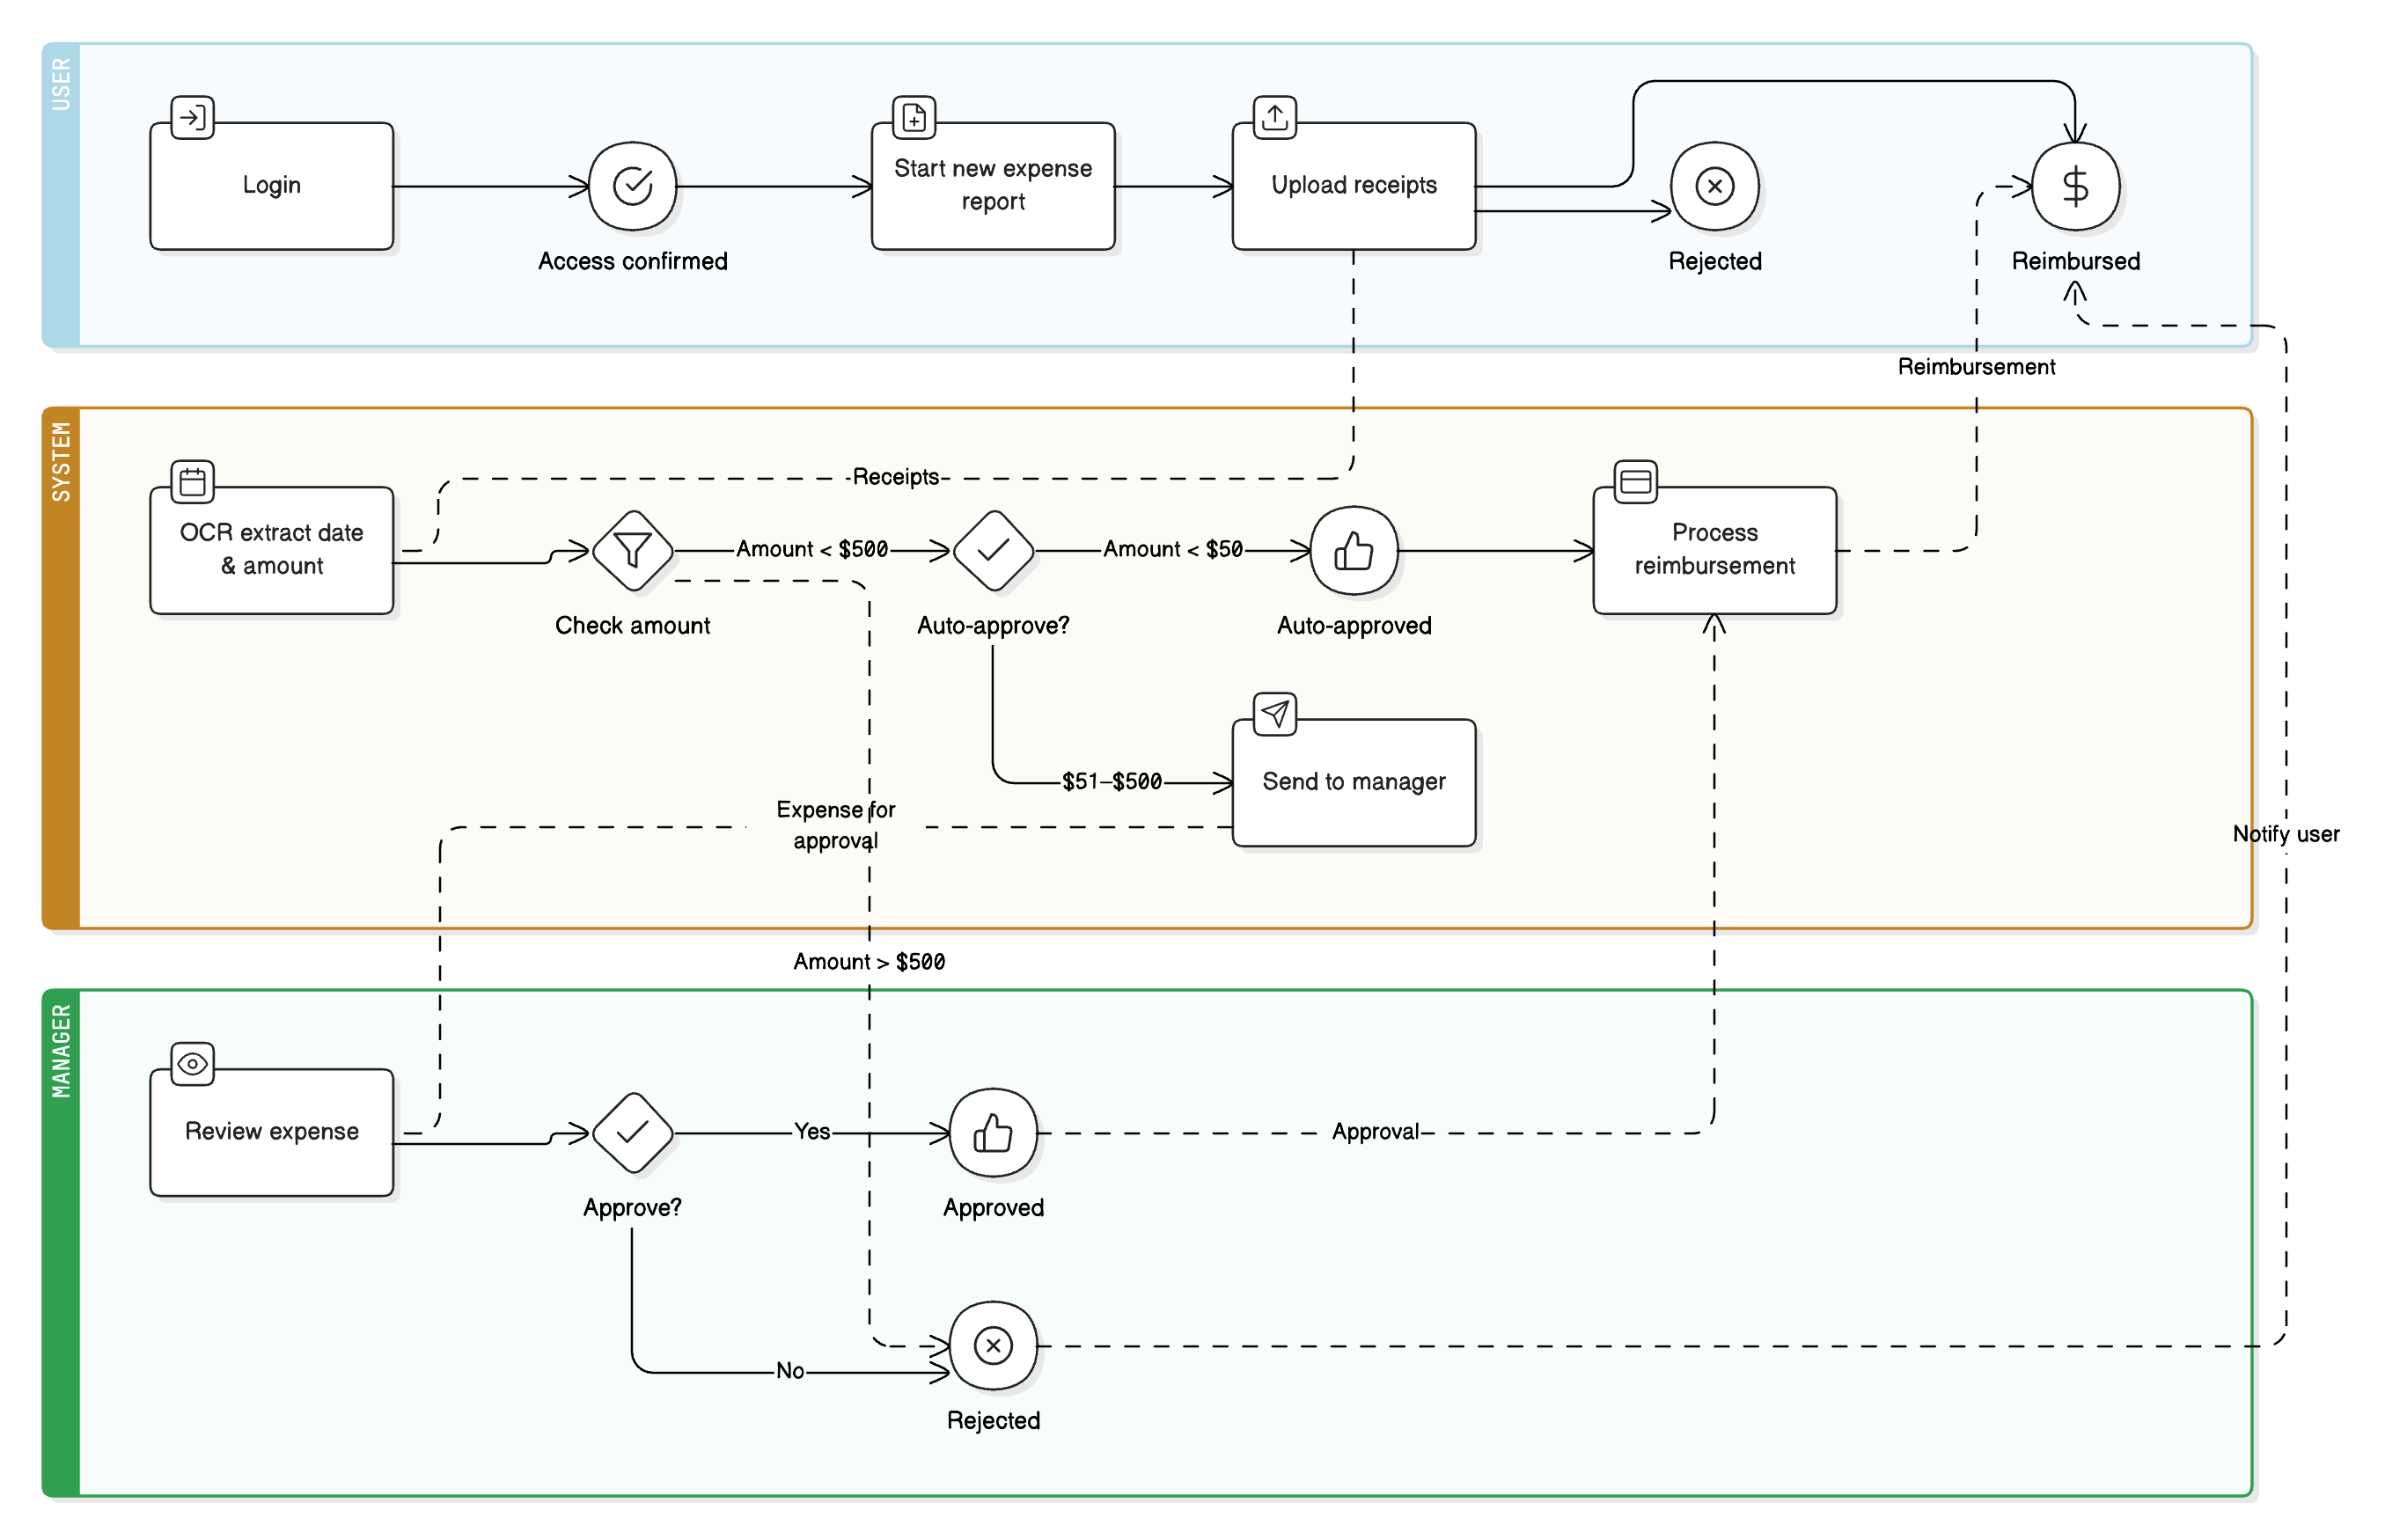
\includegraphics[width=\textwidth]{img/bpmn.png}
  \caption{BPMN diagram se swimlanes (User, System, Manager); přerušované šipky = Message Flow mezi lanes; plné šipky = Sequence Flow uvnitř lane}
\end{figure}

\noindent\textbf{Co diagramy ilustrují:}
\begin{itemize}
  \item \textbf{Start a konec} -- EPC nemá speciální symbol; první a poslední hexagon jsou implicitně
    začátek a konec. BPMN má explicitní Start Event (tenký kroužek) a End Event (tučný kroužek).
  \item \textbf{Větvení} -- EPC: kroužek s textem \textit{XOR}; BPMN: diamant s \textit{X} uvnitř --
    vizuálně odlišné, ale stejná sémantika (právě jedna větev).
  \item \textbf{Povinné střídání} -- v EPC musí po každé funkci (modrý obdélník) následovat událost
    (oranžový hexagon) -- proto jsou dva koncové hexagony. V BPMN po úkolu může rovnou následovat
    End Event bez mezivýsledkových událostí.
  \item \textbf{Orientace} -- EPC konvence: shora dolů; BPMN konvence: zleva doprava (přirozené pro swimlanes).
\end{itemize}

\paragraph{Srovnání EPC vs BPMN}

\begin{center}
\begin{tabular}{lll}
\toprule
\textbf{Aspekt} & \textbf{EPC} & \textbf{BPMN} \\
\midrule
Standard & ARIS (Prof. Scheer) & OMG standard \\
Použití & SAP projekty, ARIS tool & Obecný standard \\
Exekuce & Obtížná & BPMN 2.0 je spustitelný (BPEL) \\
Složitost & Jednodušší & Bohatší sémantika \\
Adopce & Klesá & Rostě, de facto standard \\
\bottomrule
\end{tabular}
\end{center}

\subsubsection{KBPR (Key Business Process Requirements)}

Klíčové požadavky na podnikové procesy -- rámec pro hodnocení procesů:
\begin{itemize}
  \item Efektivnost (Effectiveness) -- proces dosahuje zamýšlených výsledků
  \item Eficiencia (Efficiency) -- minimální spotřeba zdrojů
  \item Flexibilita -- schopnost adaptace na změny
  \item Bezpečnost -- ochrana informací a zdrojů
  \item Měřitelnost -- jasné metriky výkonnosti
\end{itemize}

%=============================================================================
\subsection{Architektura IS a způsoby zpracování}
%=============================================================================

\subsubsection{MDA (Model Driven Architecture)}

\textbf{OMG} (Object Management Group) -- mezinárodní nezisková standardizační organizace pro IT;
vydává standardy jako UML, BPMN, MDA. Říká se jim OMG standardy, protože za nimi stojí tato organizace.

\textbf{MDA} (OMG standard) -- přístup k vývoji SW, kde je \textbf{model} primárním artefaktem, nikoliv kód.
Myšlenka: nejprve popište systém abstraktně (co má dělat, bez technologie), pak automaticky transformujte na platformně specifický model a nakonec na kód.

\begin{itemize}
  \item \textbf{CIM (Computation Independent Model)} -- \textit{byznys pohled}; popisuje, co systém dělá z pohledu byznysu, bez jakéhokoli zmínění technologie nebo implementace; typicky BPMN diagram nebo textový popis požadavků; ``model'' zde znamená formalizovaný popis byznysu
  \item \textbf{PIM (Platform Independent Model)} -- model systému nezávislý na konkrétní platformě;
    popsán v UML; zachycuje logiku a strukturu bez technologických detailů
  \item \textbf{PSM (Platform Specific Model)} -- model přizpůsobený konkrétní platformě (Java EE, .NET, Web);
    generován transformací z PIM
  \item Z PSM lze automaticky generovat kód
\end{itemize}

Transformace: CIM $\to$ PIM $\to$ PSM $\to$ Code; každá transformace je řízenou, opakovatelnou operací.

\subsubsection{Způsoby zpracování dat v IS}

\begin{itemize}
  \item \textbf{Dávkové zpracování (Batch Processing)} -- data se shromáždí a zpracují najednou
    v určený čas (noční mzdové výpočty, měsíční výpisy); nízká latence požadavku, vysoká propustnost
  \item \textbf{Interaktivní zpracování (Online/Interactive)} -- uživatel přímo interaguje se systémem
    v reálném čase; odpověď do sekund (bankovní přepážka, rezervační systém)
  \item \textbf{Distribuované zpracování} -- výpočet rozložen na více uzlů/serverů;
    škálovatelnost, odolnost proti výpadkům; příklady: cloud, mikroservisy, Hadoop
  \item \textbf{Zpracování řízené událostmi (Event-driven)} -- komponenty reagují na události (events);
    volná vazba; příklady: IoT, mikroservisy s message brokery, GUI
  \item \textbf{Zpracování v reálném čase (Real-time)} -- striktní časové požadavky; zpracování musí
    proběhnout v definovaném čase; kritické systémy (řízení letadel, průmyslové stroje, streaming)
\end{itemize}

\paragraph{Centralizované vs. decentralizované zpracování}
\begin{itemize}
  \item \textbf{Centralizované} -- mainframe/server; jednoduchá správa, single point of failure
  \item \textbf{Decentralizované} -- výpočty u klienta; autonomie, ale složitá synchronizace
\end{itemize}

\subsubsection{Typy IS/ICT služeb}

\begin{itemize}
  \item \textbf{Informační služby} -- poskytování informací a dat (reporty, dashboardy, notifikace)
  \item \textbf{Aplikační služby} -- softwarové funkce zpřístupněné uživatelům nebo systémům (ERP, CRM, API)
  \item \textbf{Infrastrukturní služby} -- síť, servery, storage, cloud (IaaS); zajišťuje IT provoz
  \item \textbf{Podpůrné služby} -- helpdesk, service desk, školení, konzultace
\end{itemize}

\paragraph{SLA (Service Level Agreement)}
Formální smlouva definující úroveň poskytované služby:
\begin{itemize}
  \item \textbf{Dostupnost} -- např. 99.9\% uptime (8.7 hodin výpadku/rok)
  \item \textbf{Čas odezvy} -- jak rychle systém odpoví na požadavek
  \item \textbf{Čas obnovy} -- RTO (Recovery Time Objective), RPO (Recovery Point Objective)
  \item \textbf{Podpora} -- reakční doba helpdesku (P1: 1h, P2: 4h, P3: 1 pracovní den)
\end{itemize}

\begin{profesorbox}[Otázky profesorů k tématu: Analýza a návrh IS]
\textbf{Řepa Václav, prof. Ing., CSc.}
\begin{itemize}
  \item Co je MMDIS a jaké jsou jeho hlavní principy?
  \item Jaký je rozdíl mezi procesním a datovým pohledem na IS?
  \item Popište elementy EPC diagramu.
\end{itemize}
\textbf{Pour Jan, doc. Ing., CSc.}
\begin{itemize}
  \item Jaké jsou výhody BPMN oproti EPC?
  \item Co je podnikový proces a jak ho modelujeme?
  \item Jaké jsou fáze analýzy IS v MMDIS?
\end{itemize}
\textbf{Chudán David, Ing., Ph.D.}
\begin{itemize}
  \item Jaký je rozdíl mezi Sequence Flow a Message Flow v BPMN?
  \item Vysvětlete BPMN gateway typy.
\end{itemize}
\textbf{Svátek Vojtěch, prof. Ing., Ph.D.}
\begin{itemize}
  \item Co je swimlane a k čemu slouží?
  \item Jak se modeluje paralelní zpracování v BPMN a EPC?
\end{itemize}
\end{profesorbox}
